% Options for packages loaded elsewhere
\PassOptionsToPackage{unicode}{hyperref}
\PassOptionsToPackage{hyphens}{url}
%
\documentclass[
]{article}
\usepackage{amsmath,amssymb}
\usepackage{lmodern}
\usepackage{ifxetex,ifluatex}
\ifnum 0\ifxetex 1\fi\ifluatex 1\fi=0 % if pdftex
  \usepackage[T1]{fontenc}
  \usepackage[utf8]{inputenc}
  \usepackage{textcomp} % provide euro and other symbols
\else % if luatex or xetex
  \usepackage{unicode-math}
  \defaultfontfeatures{Scale=MatchLowercase}
  \defaultfontfeatures[\rmfamily]{Ligatures=TeX,Scale=1}
\fi
% Use upquote if available, for straight quotes in verbatim environments
\IfFileExists{upquote.sty}{\usepackage{upquote}}{}
\IfFileExists{microtype.sty}{% use microtype if available
  \usepackage[]{microtype}
  \UseMicrotypeSet[protrusion]{basicmath} % disable protrusion for tt fonts
}{}
\makeatletter
\@ifundefined{KOMAClassName}{% if non-KOMA class
  \IfFileExists{parskip.sty}{%
    \usepackage{parskip}
  }{% else
    \setlength{\parindent}{0pt}
    \setlength{\parskip}{6pt plus 2pt minus 1pt}}
}{% if KOMA class
  \KOMAoptions{parskip=half}}
\makeatother
\usepackage{xcolor}
\IfFileExists{xurl.sty}{\usepackage{xurl}}{} % add URL line breaks if available
\IfFileExists{bookmark.sty}{\usepackage{bookmark}}{\usepackage{hyperref}}
\hypersetup{
  pdftitle={Nanopore sequencing to analyse MGMT promoter methylation},
  pdfauthor={Skarphedinn Halldorsson},
  hidelinks,
  pdfcreator={LaTeX via pandoc}}
\urlstyle{same} % disable monospaced font for URLs
\usepackage[margin=1in]{geometry}
\usepackage{graphicx}
\makeatletter
\def\maxwidth{\ifdim\Gin@nat@width>\linewidth\linewidth\else\Gin@nat@width\fi}
\def\maxheight{\ifdim\Gin@nat@height>\textheight\textheight\else\Gin@nat@height\fi}
\makeatother
% Scale images if necessary, so that they will not overflow the page
% margins by default, and it is still possible to overwrite the defaults
% using explicit options in \includegraphics[width, height, ...]{}
\setkeys{Gin}{width=\maxwidth,height=\maxheight,keepaspectratio}
% Set default figure placement to htbp
\makeatletter
\def\fps@figure{htbp}
\makeatother
\setlength{\emergencystretch}{3em} % prevent overfull lines
\providecommand{\tightlist}{%
  \setlength{\itemsep}{0pt}\setlength{\parskip}{0pt}}
\setcounter{secnumdepth}{5}
\usepackage{fancyhdr}
\usepackage{mathtools}
\usepackage{hyperref}
\usepackage{subfig}
\setlength{\headheight}{33pt}
\setlength{\footskip}{25pt}
\pagestyle{fancy}
\renewcommand{\headrulewidth}{0.5pt}
\renewcommand{\footrulewidth}{0.5pt}
\cfoot{\scriptsize Vilhelm Magnus Laboratory | Institute for surgical research \\ Oslo University Hospital}
\rhead{\thepage}
\hypersetup{colorlinks   = true, linkcolor=blue, urlcolor  = blue}
\fancypagestyle{plain}{\pagestyle{fancy}}
\usepackage{subfig, float}
\usepackage{booktabs}
\usepackage{longtable}
\usepackage{array}
\usepackage{multirow}
\usepackage{wrapfig}
\usepackage{float}
\usepackage{colortbl}
\usepackage{pdflscape}
\usepackage{tabu}
\usepackage{threeparttable}
\usepackage{threeparttablex}
\usepackage[normalem]{ulem}
\usepackage{makecell}
\usepackage{xcolor}
\ifluatex
  \usepackage{selnolig}  % disable illegal ligatures
\fi

\title{Nanopore sequencing to analyse MGMT promoter methylation}
\usepackage{etoolbox}
\makeatletter
\providecommand{\subtitle}[1]{% add subtitle to \maketitle
  \apptocmd{\@title}{\par {\large #1 \par}}{}{}
}
\makeatother
\subtitle{Preliminary data analysis}
\author{Skarphedinn Halldorsson}
\date{Compiled on 15 desember, 2022}

\begin{document}
\maketitle

\hypertarget{introduction}{%
\subsection{Introduction}\label{introduction}}

MGMT promoter methylation is an important diagnostic factor for
glioblastoma treatment. Methylation on a CpG island in the MGMT promoter
region predicts response to the alkylating agent temozolomide. MGMT
promoter methylation is typically assessed by methylation specific PCR
(MSP) of the first exon of MGMT or pyrosequencing of 4 CpG sites in the
first exon. Both methods rely on bisulphate treatment of DNA prior to
analysis. Nanopore sequencing allows methylation calling on native,
genomic DNA. This circumvents the need for bisulphate treatment of DNA
prior to sequencing and allows methylation analysis of far larger
sequencing than either MSP or pyrosequencing.

\begin{figure}
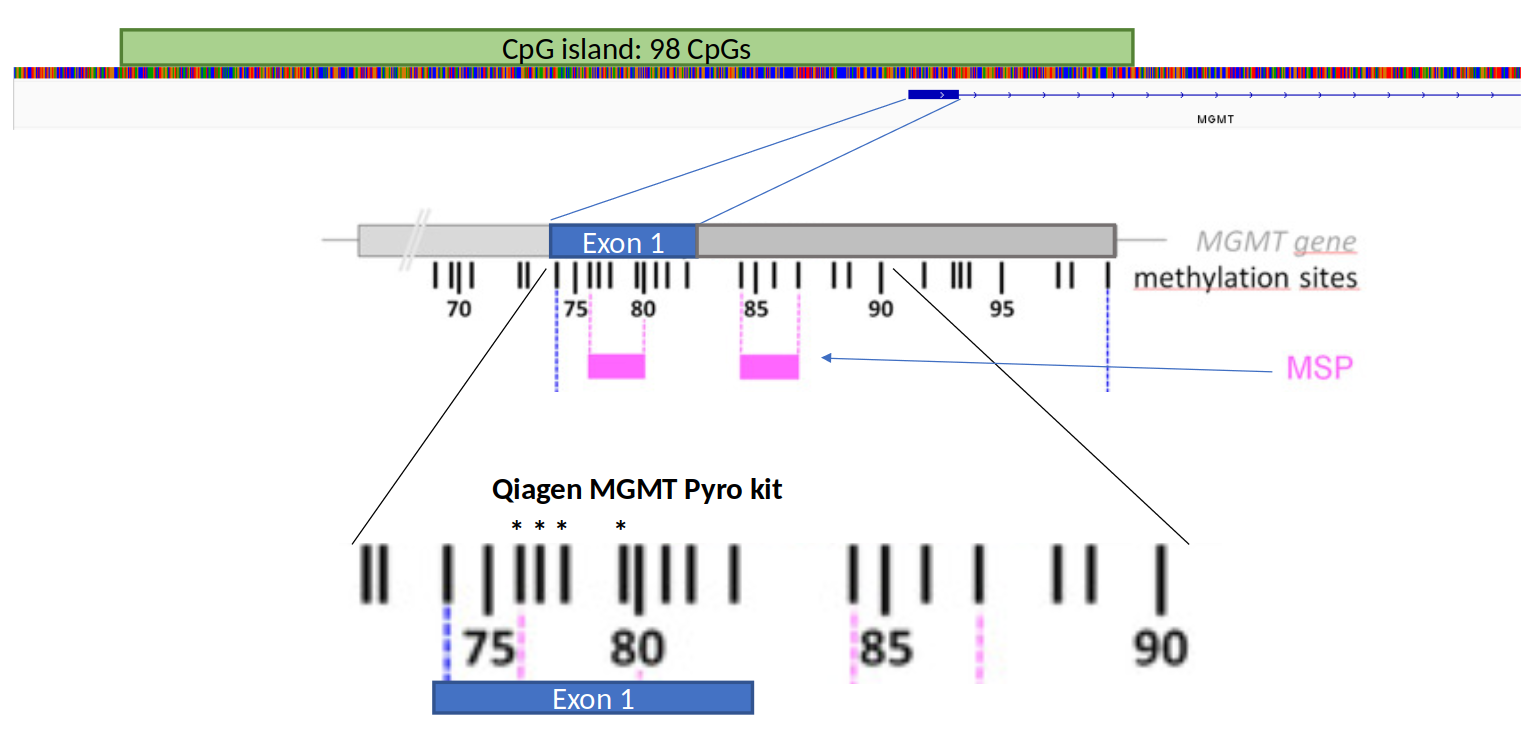
\includegraphics[width=1\linewidth]{Figures/MGMT_promoter_region} \caption{Organization of the MGMT promoter. MSP refers to the typical primer sites of methylation specific PCR to determine MGMT promoter methylation. Asterixes represent the 4 CpGs analysed by the Qiagen MGMT pyrosequencing kit.}\label{fig:Promoter}
\end{figure}

Here, we present the results of nanopore sequencing of the whole CpG
island in the promoter region of the MGMT gene. We gathered nanopore
sequencing data of the MGMT promoter region from 148 patients, including
130 glioblastoma patients. Results were produced either by CRISPR/Cas9
targeted sequencing of the MGMT promoter region or as part of an
adaptive sampling panel (RAPID-CNS). Samples were obtained from three
separate cohorts: the DenStem project at Institute for Surgical
Research, the glioblastoma DNA biobank at Radium Hospital and Rapid-CNS.
Cas9 targeted sequencing samples were either run as single samples or as
5 barcoded samples run simultaneously. An overview of samples can be
seen in Table 1.

\begin{table}

\caption{\label{tab:Sample_overview}Overview of samples included in this study}
\centering
\resizebox{\linewidth}{!}{
\begin{tabular}[t]{l|c|c|c|c|c|c|c|l}
\hline
Series & Astrocytoma & Astrocytoma HG & Glioblastoma & LGG\_PA & Meningioma & Metastasis & Oligodendroglioma & Other\\
\hline
DenStem & 3 & 0 & 13 & 0 & 0 & 0 & 0 & 0\\
\hline
Radium & 1 & 4 & 29 & 0 & 12 & 7 & 2 & 10\\
\hline
Rapid-CNS & 3 & 4 & 49 & 4 & 0 & 0 & 6 & 1\\
\hline
Total & 7 & 8 & 91 & 4 & 12 & 7 & 8 & 11\\
\hline
\end{tabular}}
\end{table}

\begin{figure}
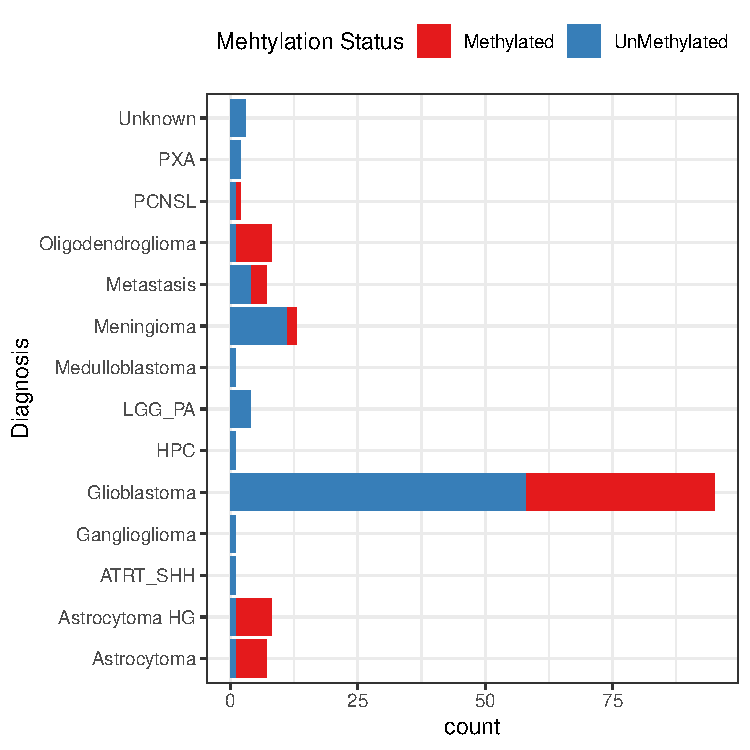
\includegraphics[width=0.75\linewidth]{Nano-MGMT_files/figure-latex/Methylation_overview-1} \caption{Distribution of methylated versus unmethylated samples as measured by pyrosequencing}\label{fig:Methylation_overview}
\end{figure}

\hypertarget{data-acquisition}{%
\subsection{Data acquisition}\label{data-acquisition}}

Figures 3 and 4 show the sequencing depth of samples in this study.
Figure 3 shows that there is no implicit bias between methylated versus
unmethylated samples when it comes to sequencing depth. Figure 3 shows
that the range of depth is large. Single sample runs produce more
sequences than barcoded runs, adaptive sampling similar sequencing depth
as barcoded Cas9 targeted samples.

\begin{figure}
\centering
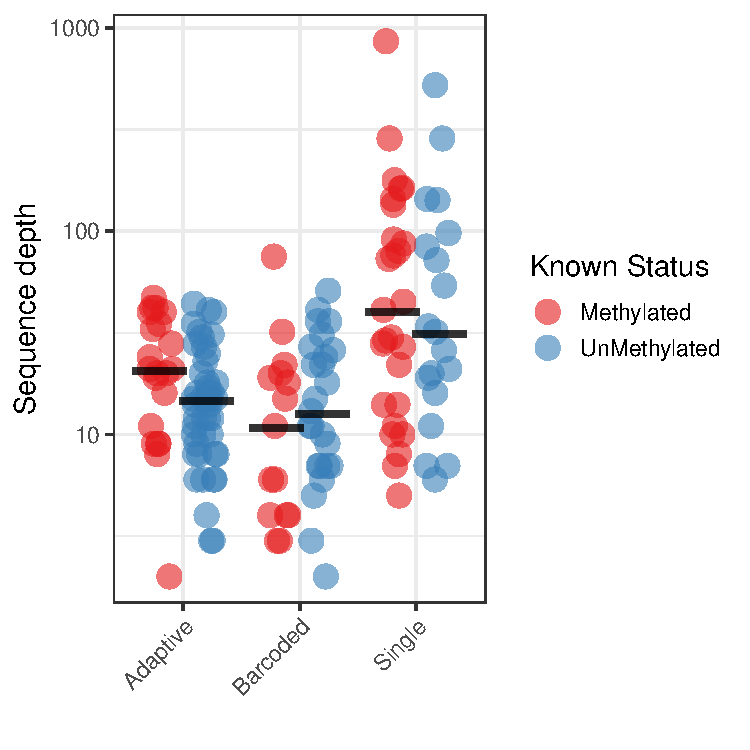
\includegraphics{Nano-MGMT_files/figure-latex/Coverage_Method-1.pdf}
\caption{Sequencing depth of samples by method of acquisition, group
median represented by red diamond. No bias in sequence depth observed
between methylated and unmethylated samples.}
\end{figure}

\begin{figure}
\centering
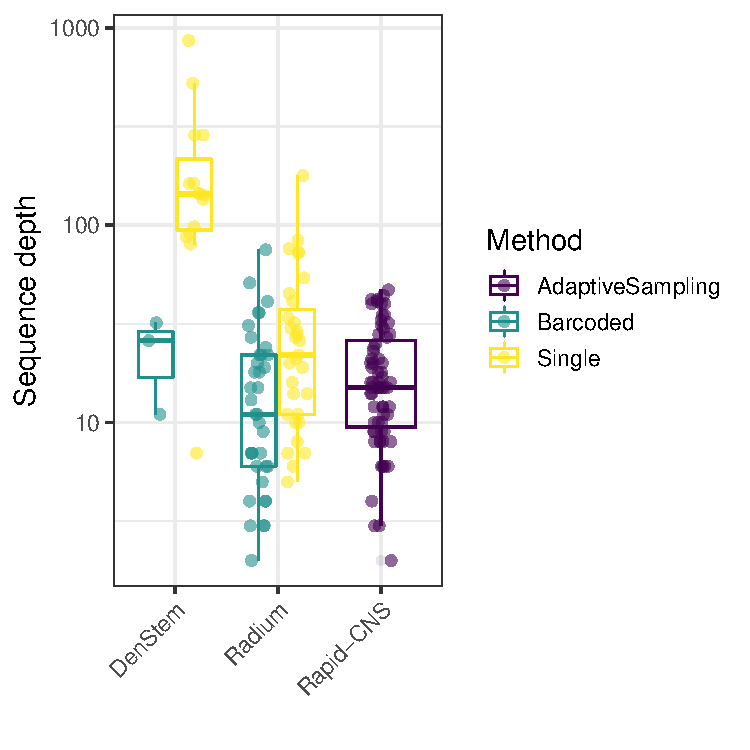
\includegraphics{Nano-MGMT_files/figure-latex/Coverage_Dataset-1.pdf}
\caption{Sequencing depth of methods, group median represented by red
diamond. Single sample runs generally have higher sequence depth than
barcoded samples or adaptive sampling.}
\end{figure}

\hypertarget{direct-comparison-of-nanopore-sequencing-and-pyrosequencing}{%
\subsection{Direct comparison of Nanopore sequencing and
Pyrosequencing}\label{direct-comparison-of-nanopore-sequencing-and-pyrosequencing}}

At the Norwegian University hospital, MGMT promoter methylation is
determined by the Qiagen MGMT pyrosequencing kit. Results are typically
presented as an avererage methylation percentage across the four CpGs
detected by the kit. A cut-off value of 9\% determines if a given sample
is classified as ``methylated'' or ``unmethylated''. We currently have
average methylation values for the DenStem samples and the Radium
samples (Figure 5).

\begin{figure}
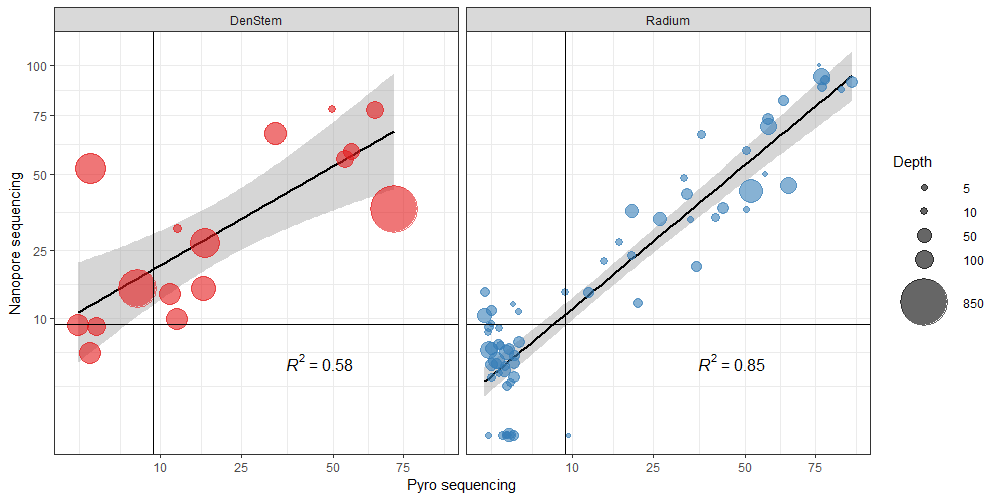
\includegraphics[width=1\linewidth]{Nano-MGMT_files/figure-latex/Compare_Group-1} \caption{Comparison of nanopore sequencing and Pyrosequencing results of 4 CpGs in exon 1 of the MGMT promoter. Plotted values are average methylation of 4 CpGs. Black horizontal and vertical lines mark the 9 percent cut-off value between methylated and unmethylated samples, as determined by pyrosequencing.}\label{fig:Compare_Group}
\end{figure}

Plotting the average methylation percentage acquired via Nanopore
sequencing against the values acquired by pyrosequencing shows
reasonable correlation between the two methods, particularly for the
Radium samples (R\textsuperscript{2}=0.85). It should be noted that the
DenStem results are from the same tumor but not the same biopsy (one
biopsy for nanopore, another biopsy for pyrosequencing) while the Radium
samples are from the same biopsy (same biopsy analysed by nanopore
sequencing and pyrosequencing). This is a likely explanation of why the
correlation between nanopore sequencing and pyrosequencing is lower in
this cohort. This also raises the question of heterogeneity of
methylation status throughout a tumor entity, especially if methylation
\% is close to the cut-off value. Would a different biopsy have slightly
higher or lower methylation values that might classify the tumor
differently? I don't think the DenStem samples presented here can really
answer that as they were analysed by different methods but it's worth a
thought.

There appears to be a certain level of over-prediction of methylation \%
by nanopore sequencing compared to the pyrosequencing results,
particularly in low methylation samples. This means that the \%
methylated cut-off value for nanopore sequencing is higher than the 9 \%
methylated threshold that is applied for pyrosequencing. These results
only apply for the 4 CpGs sequenced by the Qiagen MGMT pyrosequencing
kit. It should also be notet that \% methylated values in very low
coverage samples are unreliable.

\begin{figure}
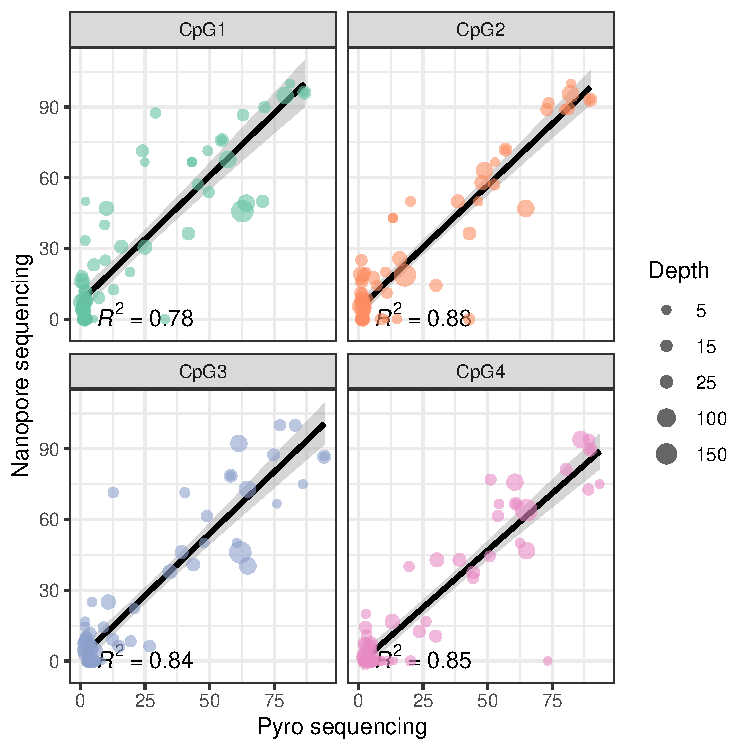
\includegraphics[width=1\linewidth]{Nano-MGMT_files/figure-latex/Compare_Individual-1} \caption{Comparison of individual CpGs within exon 1}\label{fig:Compare_Individual}
\end{figure}

We also have separate methylation percentage values for the four CpGs
analysed by the Qiagen MGMT pyrosequencing kit for all the Radium
samples. This affords a site by site comparison between nanopore
sequencing and pyrosequencing (Figure 6). The correlation between
nanopore and pyrosequencing is slightly less for the individual CpGs a
difference that appears to be rounded out when the values are averaged
(Figure 5, Radium).

Take together, nanopore sequencing of the same 4 CpGs analysed by the
Qiagen MGMT pyrosequencing kit does a reasonable job of recreating the
pyrosequencing results. However, this does not take advantage of the
other 94+ CpGs that are included in the nanopore data.

\hypertarget{unsupervised-clustering-of-nanopore-results}{%
\subsection{Unsupervised clustering of nanopore
results}\label{unsupervised-clustering-of-nanopore-results}}

\begin{figure}
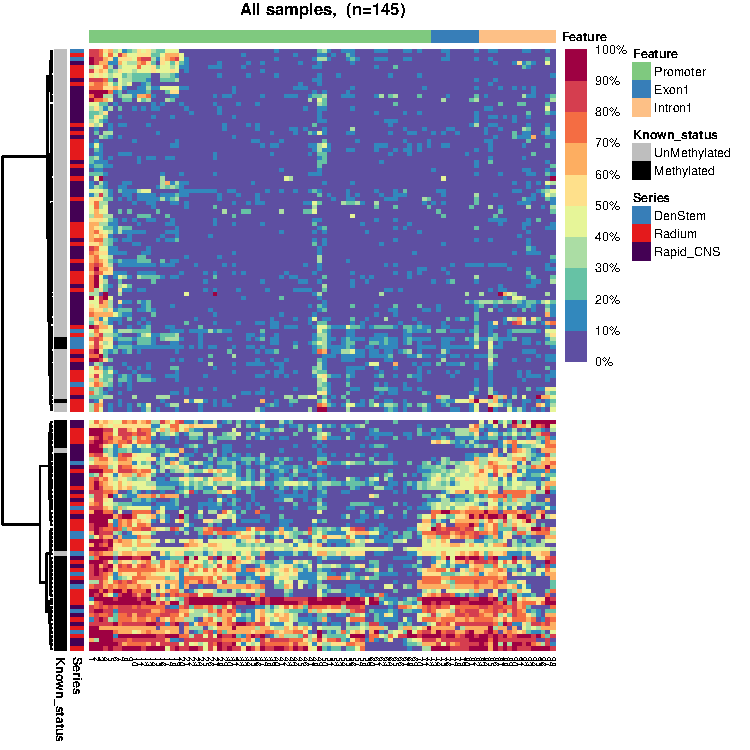
\includegraphics[width=1\linewidth,height=1.2\textheight]{Nano-MGMT_files/figure-latex/Heatmap-1} \caption{Clustered heatmap of all samples based on nanopore sequencing of CpG island of the MGMT promoter}\label{fig:Heatmap}
\end{figure}

Unsupervised clustering of all the samples included in the study shows
very clear separation of methylated and unmethylated samples (Figure 7).
The samples previously defined as unmethylated have very low methylation
throughout the CpG island apart from the first 5 CpGs that are often
methylated. Samples previously defined as methylated have a gradient of
methylation which tends to show highest methylation values towards
either end of the CpG island. Only six samples samples do not cluster
according to their previously determined methylation status. Four of
these samples belong to the DenStem cohort that is not directly
comparable, as previously mentioned. A single sample from the Radium
cohort was classified as methylated by pyrosequencing but clusters with
the unmethylated samples. This sample is interesting as it has robust
methylation in the fist exon but very low methylation elsewhere in the
CpG island.

We can also look at methylation patterns specifically in the
glioblastoma samples (Table 1).

\begin{figure}
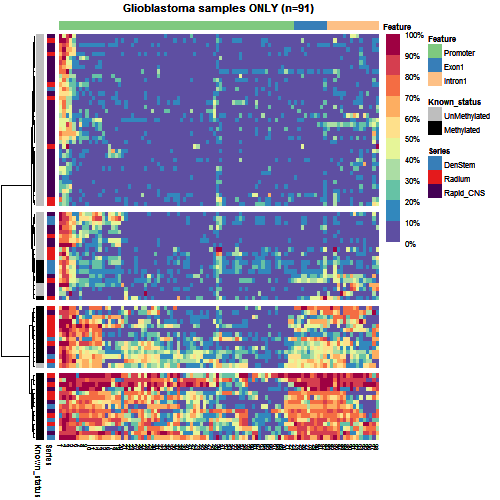
\includegraphics[width=1\linewidth,height=1.2\textheight]{Nano-MGMT_files/figure-latex/HeatmapGBM-1} \caption{Heatmap showing unsupervised clustering of glioblastoma samples based on nanopore sequencing of the CpG island in the MGMT promoter}\label{fig:HeatmapGBM}
\end{figure}

In Figure 8 we see that all of the Rapid-CNS GBM samples fall within
their previously determined classes and only one of the Radium samples
is ``mis-classified''. We also see there are clusters within both the
methylated and unmethylated samples. These clusters can also be
represented by mean methylation values within each cluster (Figure 9).

\begin{figure}
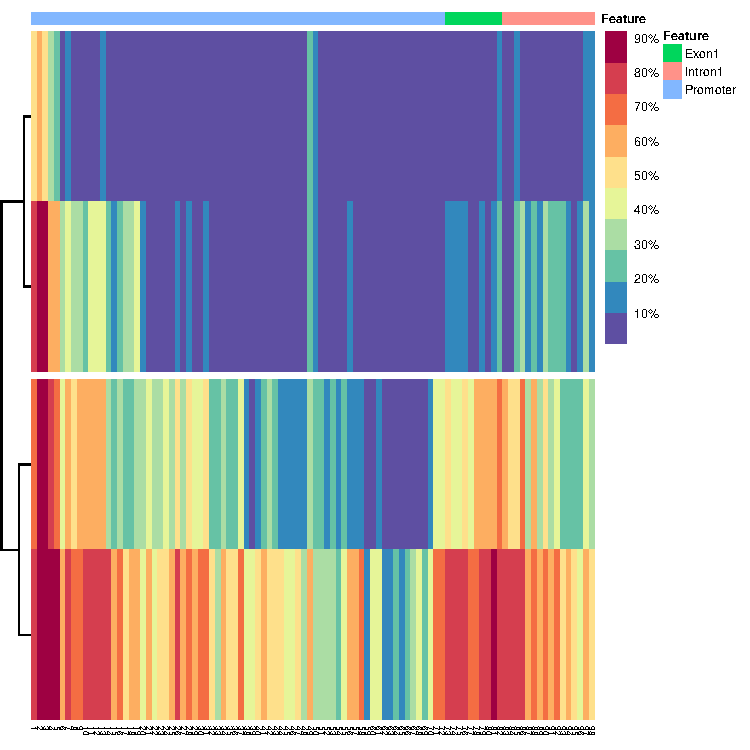
\includegraphics[width=1\linewidth,height=1.2\textheight]{Nano-MGMT_files/figure-latex/Kmeans-1} \caption{K-means clustering of glioblastoma samples}\label{fig:Kmeans}
\end{figure}

\hypertarget{discussion}{%
\subsection{Discussion}\label{discussion}}

We have a fairly extensive dataset of 153 samples, including 91 GBMs.
I've not seen data with this many samples that looks at methylation
within the whole CpG island of MGMT. We have the option of looking for
CpG methylation further upstream and downstream than the 98 CpG
presented here, at least 10 CpGs in both directions without losing any
samples due to lack of coverage. By focusing on high depth samples we
can look much further. I have not included that here but will be looking
into it and will report if I find anything interesting.

We can conclude that nanopore sequencing of the MGMT promoter region
performs as well or better than standard methods such as pyrosequencing.
This is true for both cas9 targetted sequencing of the MGMT promoter and
inclusion of the MGMT promoter into an adaptive sequencing panel.
Distinct subgroups within both methylated and unmethylated samples are
captured via nanopore sequencing, it will be very interesting to see if
there is a difference in patient outcome between these clusters.

\end{document}
